\section{Characteristics of the fluctuations}
As seen in \cref{fig:2DFluct} the fluctuations can be quite strong, something which has also been observed experimentally in for example \cite{Burin2005}.
This is something which need to be considere when modelling the plasma.
Models like Hasegawa-Wakatani \cite{Hasegawa1987,Holland2007} are doing a split between background and fluctuations.
%
\begin{wrapfigure}{l}{0.50\textwidth}
    \begin{center}
    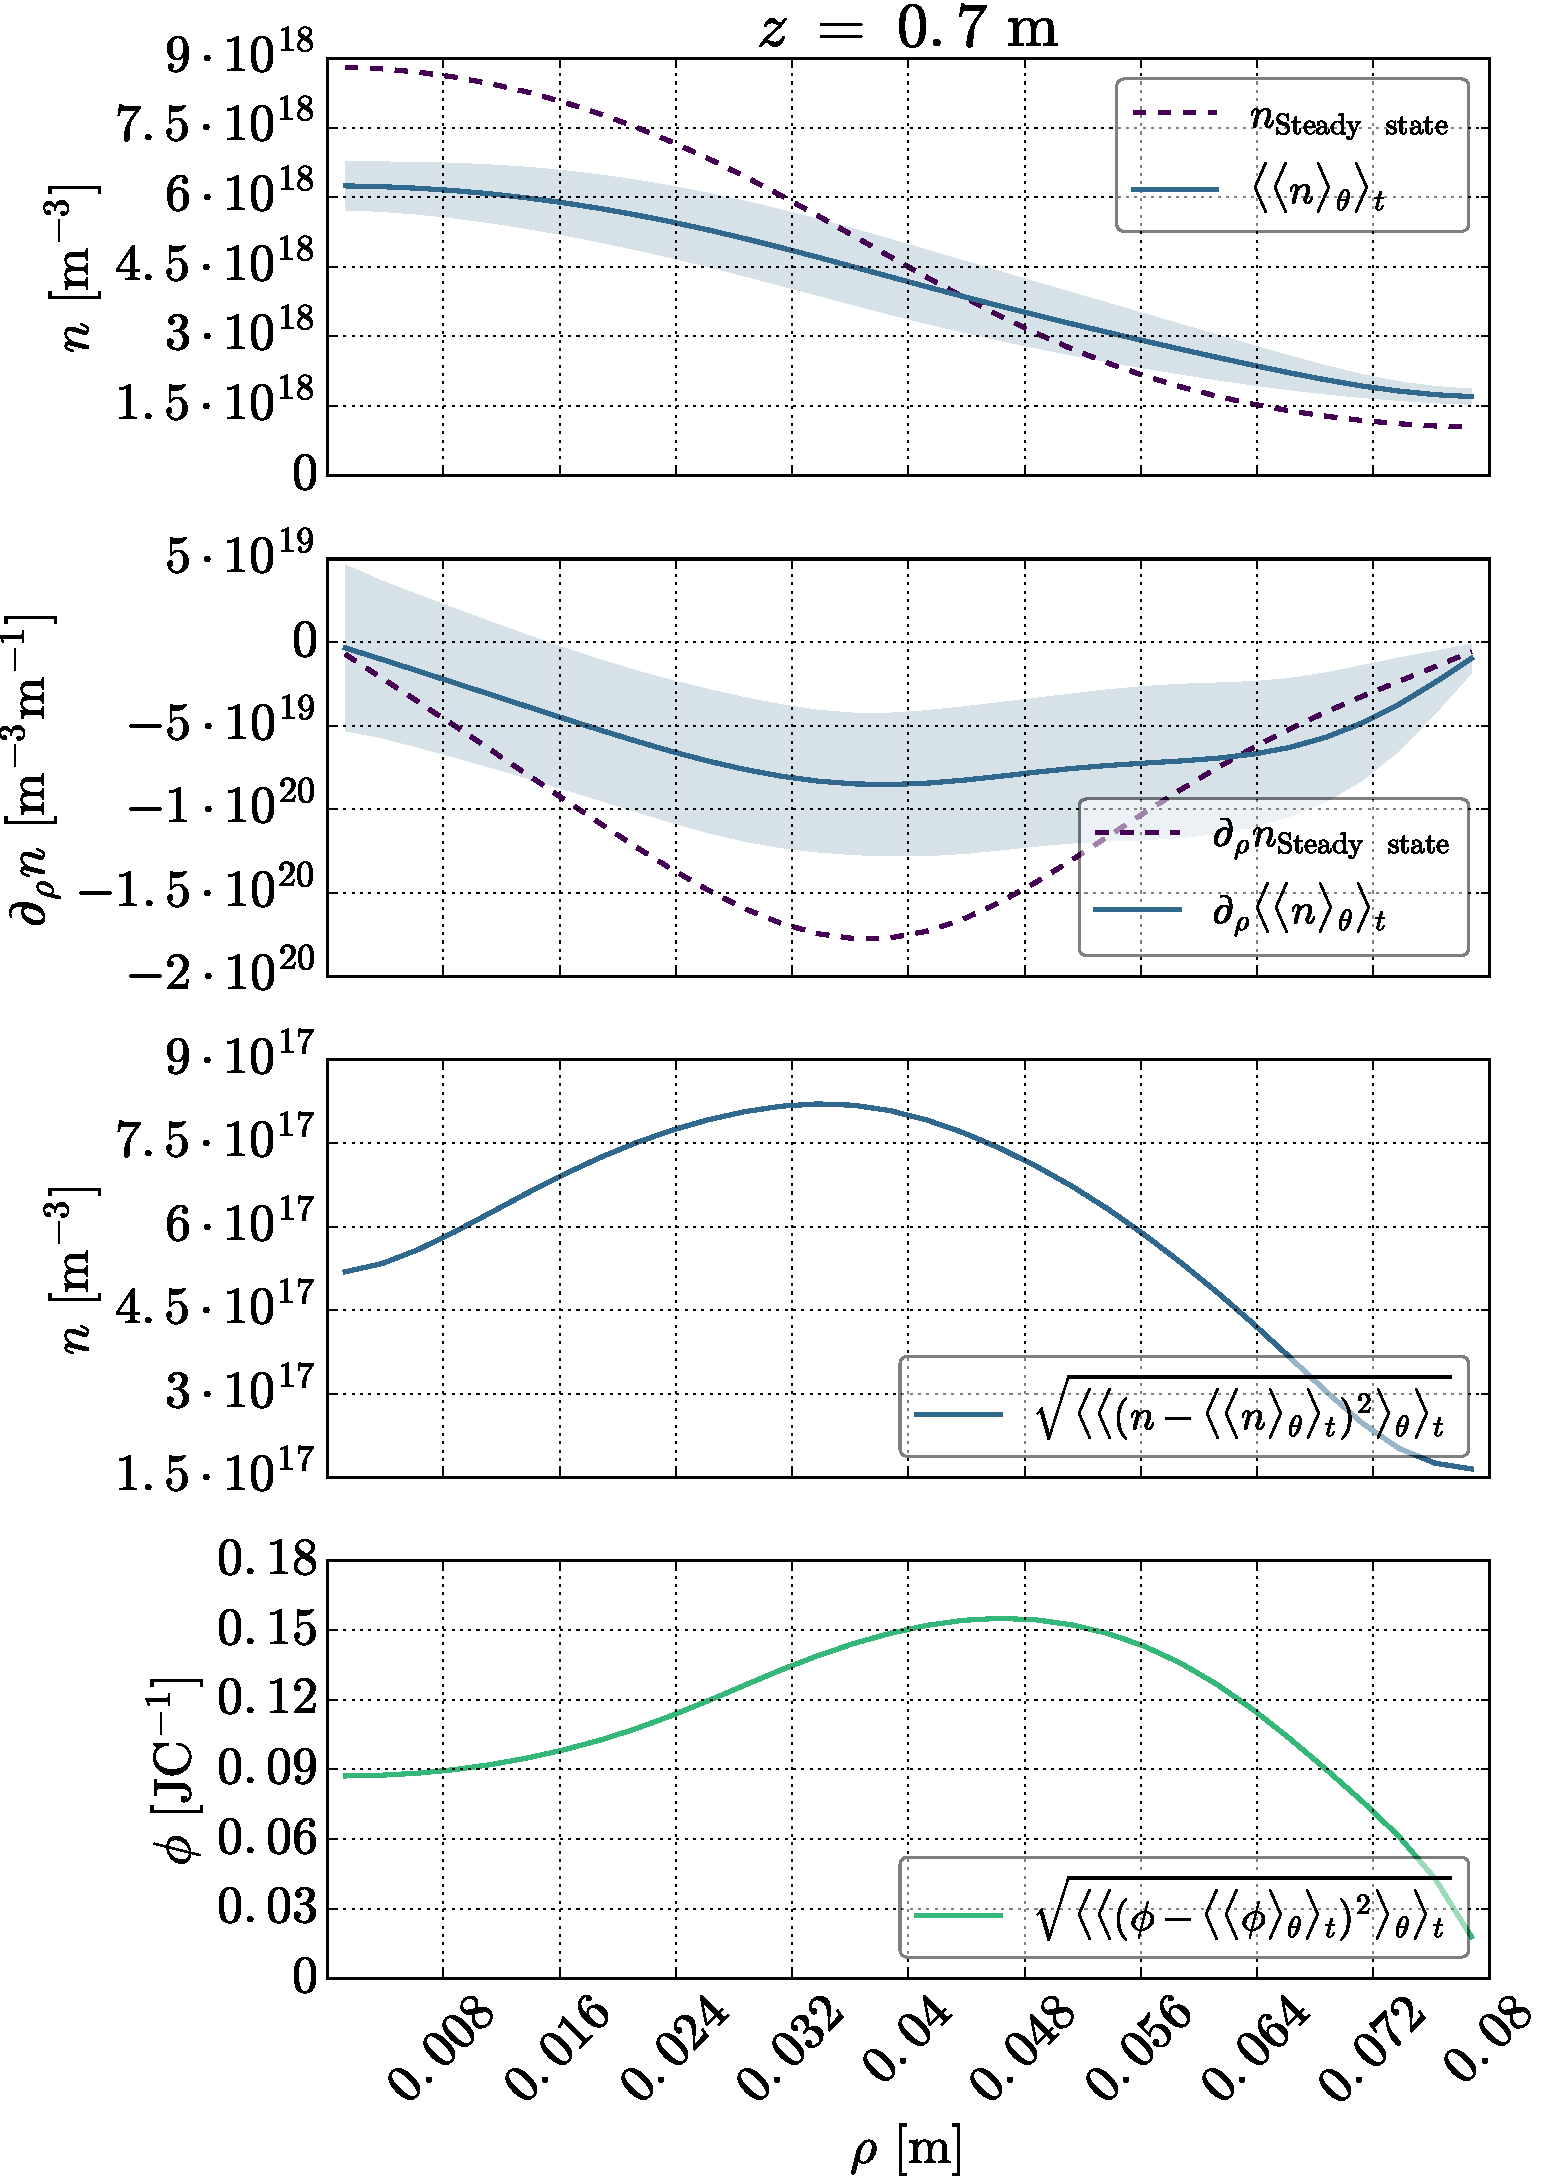
\includegraphics[width=0.48\textwidth]{fig/results/posOfFluct/posOfFluctB008}
    \end{center}
    \caption{Flattening of the profiles together with the position of the fluctuations for $B=0.08\T$.
        The shaded area represents the standard deviation.
    }
    \label{fig:posOfFluct008}
\end{wrapfigure}
%
In such models, the free energy in the background gradients are driving the fluctuations, and the feedback of the fluctuation on the background profiles are neglected.
This is good approximation if the fluctuations are small.
Nontheless, if the fluctuations are large, the background gradients are altered, and is the drive for the fluctuations.
Models like CYTO \cite{Naulin2008,Windisch2011a,Windisch2011b} and CELMA does not do this separation, and one is able to investigate how the fluctuations affect the background.
The comparison can be done by comparing the steady state profiles with the turbulent profiles, as shown in \cref{fig:posOfFluct008}.
Here, a poloidal and temporal average (containing the whole time series) have been done in order to get a good avergaged picture of the turbulent profile.
As apparent from figure \cref{fig:posOfFluct008} the background profiles are flattened by the turbulence.

FIXME: Consider to include the type of fluctuation present.
Mention Jassby position of fluctuations.
NOTE: INSERT LINEAR THEORY AND LOCATION OF FLUCTUATIONS
%
\begin{figure}[htb]
    \centering
    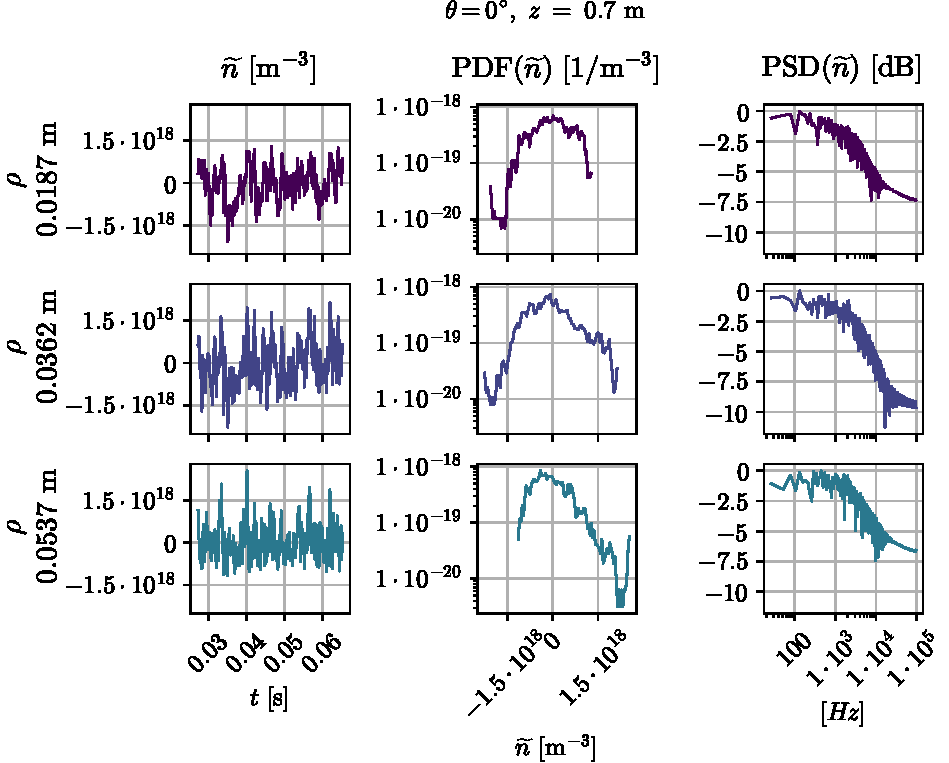
\includegraphics[width=1.0\textwidth]{fig/results/combinedPlots/008T}
    \caption{Characteristics of the time traces of the fluctuations at three radial positions.
        The top row shows data probed close to the edge of the plasma,
        the middle row shows data probed at position of the highest density gradient,
        and the bottom shows data probed close to the axis of the cylinder.
    }
    \label{fig:combinedPlots008}
\end{figure}
%
%
\begin{wrapfigure}{r}{0.5\textwidth}
    \begin{center}
        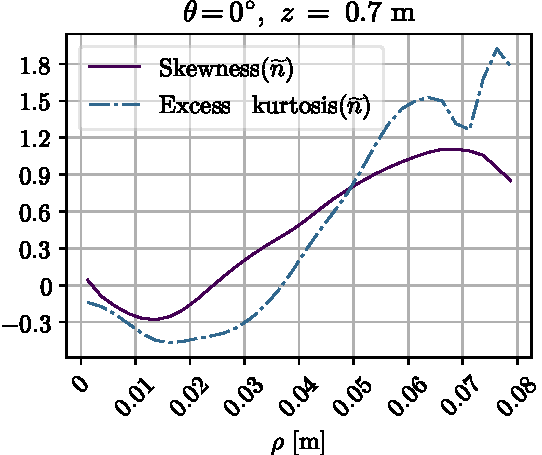
\includegraphics[width=0.48\textwidth]{fig/results/skewKurt/008T}
    \end{center}
    \caption{Radial variations of the skewness and excess kurtosis (the kurtosis $-3$).}
    \label{fig:skewKurt008}
\end{wrapfigure}
%
Further investigation of the turbulence can be done using the time traces at a fixed point.
This is done in \cref{fig:combinedPlots008}.

Again, we can observe that the fluctuations are large in amplitude, and increasingly intermittent for higher radius.
The power spectra density (PSD) shows that several frequencies are present simultaneously, and that the system is more turbulent at the edge.
This behavior is captured by the probability density functions (PDF), which measures the chance to encounter a value within an infinitesimal range, if a value at a random time is withdrawn from the time trace.
Consequentially, if all values are equally probable, the PDF will have a Gaussian shape.
Deviations from the Gaussian shape is usually measured by the statistical moments skewness%
%
\footnote{
    The skewness is a measure of the mass of the distribution.
    If the skewness is negative, the left tail of the distribution is bigger than the right.
    For a pure Gaussian the skewness is 0.
}
%
and kurtosis
%
\footnote{
    The kurtosis is a measure of extreme events present in the distribution.
    For a pure Gaussian the skewness is 3.
    If the kurtosis is less than 3 (platykurtic) the distribution produces fewer and less extreme outliers than a Gaussian.
    If the kurtosis is greater than 3 (leptokurtic) there are more extreme outliners, and the tails approaches zero slower than a Gaussian.
}
%
.
Figure \cref{fig:skewKurt008} highlights how this varies with the radius.
One can see that close to the center, it is more probable to encounter a large negative fluctuation than a positive fluctuation.
Then, for higher radii, large positive fluctuations becomes more and more frequent.
From the excess kurtosis, we can see that extreme events are less likely than in a Gaussian random process, whereas extreme events are almost twice as likely in the edge as in a Gaussian random process.

Finally it can be noted that the radial turbulent transport is mainly positive and even more intermittent than the fluctuations in density alone.
